\begin{exo}
	À la bataille navale, chaque joueur a une flotte composée de cinq bateaux : un porte-avions (5 cases), un croiseur (4 cases), un contre-torpilleur (3 cases), un sous-marin (3 cases) et un torpilleur (2 cases).

	Un joueur a disposé ses bateaux comme représentés ci-après. Les bateaux sont obligatoirement disposés horizontalement ou verticalement.

	\begin{center}
		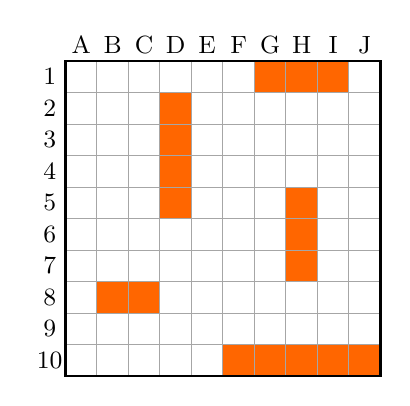
\begin{tikzpicture}[scale=0.4]
			\foreach \x/\label [count=\i] in {1/A, 2/B, 3/C, 4/D, 5/E, 6/F, 7/G, 8/H, 9/I, 10/J} { \node at (\i - 0.5, 10.5) {\small \label}; }
			\foreach \y [count=\i] in {1, 2, 3, 4, 5, 6, 7, 8, 9, 10} { \node at (-0.5, 10.5 - \i) {\small \y}; }
			\draw[gray!70, thin] (0,0) grid (10,10);
			\draw[thick] (0,0) rectangle (10,10);
			\fill[orange!80!red] (6,9) rectangle (9,10);
			\fill[orange!80!red] (3,5) rectangle (4,9);
			\fill[orange!80!red] (7,3) rectangle (8,6);
			\fill[orange!80!red] (1,2) rectangle (3,3);
			\fill[orange!80!red] (5,0) rectangle (10,1);
			\draw[gray!70, thin] (0,0) grid (10,10);
			\draw[thick] (0,0) rectangle (10,10);
		\end{tikzpicture}
	\end{center}

	L'autre joueur choisit de tirer sur une case au hasard.
	\begin{enumerate}
		\item Quelle est la probabilité qu'il touche un bateau ?
		\item Quelle est la probabilité qu'il touche un bateau s'il décide de ne tirer que dans les colonnes D et H ?
		\item Au tour précédent, il a touché la case D4. Quelle est la probabilité de toucher à nouveau le croiseur en jouant correctement ?
	\end{enumerate}
\end{exo}
